\section{Decentralized Algorithm with Partial Information}
Generally speaking, the optimal policy could be obtained by solving the minimization problem on the right-hand-side of the above Bellman's equation Eqn. (\ref{eqn:sp_0}).
In our problem, however, the GSI is not available and the centralized agent design is impractical due to randomness of \brlatency.
On the other side, conventional value iteration algorithm is intractable due to the tremendous state space.
The number of system states and action space would grow exponentially with respect to the number of APs and edge servers.
In this section, we propose a low-complexity solution scheme where each AP updates its dispatching policy according to its OSI in an iterative manner.

\subsection{Low-Complexity Solution Framework}
\begin{figure}[htp!]
    \centering
    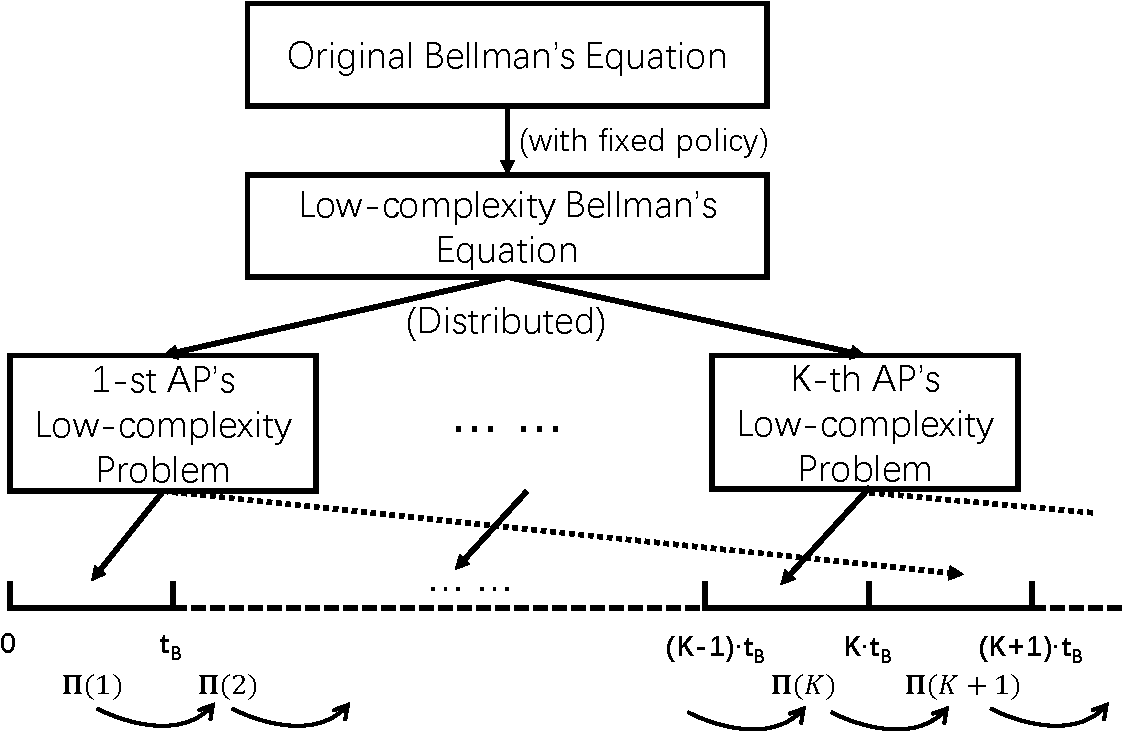
\includegraphics[width=0.45\textwidth]{images/solution-framework.pdf}
    \caption{The illustration of how low-complexity solution framework works over timeline.}
    \label{fig:solution}
\end{figure}
The whole picture of our low-complexity solution scheme is depicted in Fig.\ref{fig:solution}.

We firstly show that the right-hand-side of the original Bellman's equation could be approximated by introducing \emph{fixed policy}.
The \emph{fixed policy} is state-invariant and thus we could solve the minimization problem on right-hand-side directly.
Furthermore, we decouple the minimization problem over joint policy $\Policy(\Stat(t))$ into $K$-sub problems, where the $k$-th sub-problem aims at minimizing the cost with individual policy $\Omega_{k}(\Obsv_{k}(t))$ over OSI $\Obsv_{k}(t)$.

Then, we update the individual policy of the $k$-th AP ($\forall k\in\apSet$) at one time in an iterative manner, where the policy adapted in the previous interval is taken as \emph{fixed policy} input of the next interval.
Hence, we denote the \emph{fixed policy} in each interval as follows.
\begin{definition}[Time-variant Fixed Policy]
    \begin{align}
        \Baseline(t) \define \Bracket{\Pi_{1}(t), \dots, \Pi_{K}(t)},
    \end{align}
    where $\Pi_{k}(t) \define \set{\pi_{k,j}(t) | \forall j\in\jSpace}$ ($\forall k\in\apSet$).
\end{definition}
Specifically, we have a heuristic selfish policy as the initial policy $\Baseline^{\dagger}$ whose definition is given as follows.
\begin{definition}[Selfish Policy]
    \begin{align}
        \Baseline^{\dagger} &\define \Bracket{ \Pi^{\dagger}_{1}, \dots, \Pi^{\dagger}_{K} }
        \\
        \pi^{\dagger}_{k,j} \define \arg\min_{m} \mathbb{E}[U_{k,m,j}] + \mathbb{E}[C_{m,j}]
    \end{align}
\end{definition}

The details of the procedure is elaborated as follows.
\begin{itemize}
    \item Choose the initial policy start with the heuristic selfish policy defined above:
    \begin{align*}
        \Baseline(0) \gets \Baseline^{\dagger}
    \end{align*}

    \item For $t\in[0, 1)$, the AP indexed with $1$ would receive the OSI $D_1(1)$ time slots after the $1$-st broadcast, and then it updates its own $\Pi_{1}(1)$ by calling the function:
    \begin{align*}
        \Pi_{1}(1) \gets \algname(k, \Baseline(0)).
    \end{align*}
    Then the new fixed policy $\Baseline(1)$ is obtained by composing $\Pi_{1}(1)$ as follows.
    \begin{align*}
        \Baseline(1) \gets \Bracket{\Pi_{1}(1), \Pi_{2}(0), \dots, \Pi_{K}(0)}.
    \end{align*}

    \item Similarly, when $t\in[i, i+1]$, the AP indexed with $k' \equiv (i + 1)\mod{K}$ would receive the OSI $D_{k'}$ time slots later, and then it updates its own $\Pi_{k'}(i+1)$ by calling the function:
    \begin{align*}
        \Pi_{k'}(i+1) \gets \algname(k', \Baseline(i)).
    \end{align*}
    Then the new fixed policy $\Baseline(i+1)$ is obtained by composing $\Pi_{k'}(i=1)$ as follows.
    \begin{align*}
        \Baseline(i+1) \gets \Bracket{\Pi_{1}(i), \dots, \Pi_{k'}(i=1), \dots, \Pi_{K}(i)}.
    \end{align*}
\end{itemize}
The explicit definition of the function $\algname$ is given in the following sections.
%----------------------------------------------------------------------------------------%

\subsection{Value Function Analysis and Approximation}
In this sub-section, we elaborate the method to approximate the original Bellman's equation.

Firstly, we notice that the transition function in Eqn.(\ref{eqn:sp_0}) could be rewrite in the following form.
\begin{align}
    & \Pr\Brace{ \Stat(t+1)|\Stat(t), \Policy(\Stat(t)) }
    \nonumber\\
    =& \prod_{j\in\jSpace}\prod_{k\in\apSet}\prod_{m\in\esSet}
            \Pr\Brace{
                \vec{R}^{(k)}_{m,j}(t+1) | \vec{R}^{(k)}_{m,j}(t),
                \set{\omega_{k,j}(t), \omega_{k,j}(t+1)}
            }  
        \nonumber\\
        & \times \prod_{j\in\jSpace}\prod_{m\in\esSet}
            \Pr\Brace{
                Q_{m,j}(t+1)|Q_{m,j}(t), \mathcal{R}(t),
                \set{\omega_{k,j}(t), \omega_{k,j}(t+1)|\forall k\in\apSet}
            },
\end{align}
where the transition function is decoupled into two parts of state transition on APs and edge servers, respectively.
To efficiently express the state transition, we further elaborate the distribution probability of the state vector as the corresponding probability vector, and perform the state transition with the transition matrix.

%NOTE: transition matrix and vector for AP
For state transition of APs inside one interval, we denote $\vecG{\Theta}^{(k)}_{m,j}(t,n)$ and ${\Gamma}^{(k)}_{m,j}(t,n)$ as probability vector and transition matrix, respectively.
\begin{definition}[Denotation of Transition on AP]
    The definition for $\vec{R}^{(k)}_{m,j}(t,n)$ of the $j$-th type of job uploading from the $k$-th AP to the $m$-th edge server ($\forall k\in\apSet, m\in\esSet, j\in\jSpace$) is given as follows.
    \begin{align}
        \Gamma^{(k)}_{m,j}(t,n) \define
        \begin{bmatrix}
            1 & \bar{p}^{(k)}_{m,j,0} &                       &        &                           \\
            & 0                     & \bar{p}^{(k)}_{m,j,1} &        &                           \\
            &                       & \ddots                & \ddots &                           \\
            &                       &                       & \ddots & \bar{p}^{(k)}_{m,j,\Xi-1} \\
            &                       &                       &        & 0                         \\
        \end{bmatrix},
        \vecG{\Theta}^{(k)}_{m,j}(t,n) \define
        \begin{bmatrix}
            \theta^{(k)}_{m,j,0}(t,n) \\
            \theta^{(k)}_{m,j,1}(t,n) \\
            \vdots \\
            \vdots \\
            \theta^{(k)}_{m,j,\Xi}(t,n)
        \end{bmatrix},
    \end{align}
    where $p^{(k)}_{m,j,\xi} \define \Pr\{U^{(k)}_{m,j} < (\xi+1) | U^{(k)}_{m,j}>\xi\}$ and $\bar{p}^{(k)}_{m,j,\xi} = 1 - p^{(k)}_{m,j,\xi}$ denote the probability of staying and offloading, respectively; $\theta^{(k)}_{m,j,\xi}(t,n) \define \Pr\{R^{(k)}_{m,j,\xi}(t,n) = 1\}$ denotes the distribution probability of existing job in the corresponding counters of the AP ($\forall \xi=0,\dots,\Xi$).

    And we note that $\theta^{(k)}_{m,j,0}(t,n)$ is purely determined by the arrival process and dispatching policy of the $j$-th type of job on the $k$-th AP, i.e. $\theta^{(k)}_{m,j,0}(t,n) = \lambda_{k,j} I[\omega_{k,j}(t,n) = m]$, where $I[\cdot]$ is the indicator function.
    Hence, the state transition between adjacent interval from $\vecG{\Theta}^{(k)}_{m,j}(t+1)$ to $\vecG{\Theta}^{(k)}_{m,j}(t)$ is composed of two-phase policy separated by $D_k(t)$, which could be expressed as follows.
    \begin{align}
        \vecG{\Theta}^{(k)}_{m,j}(t, D_{k}(t)) &= (\Gamma^{(k)}_{m,j})^{D_{k}(t)} \times \vecG{\Theta}^{(k)}_{m,j}(t),
        \nonumber\\
        \vecG{\Theta}^{(k)}_{m,j}(t+1) &= (\Gamma^{(k)}_{m,j})^{N-D_{k}(t)} \times \vecG{\Theta}^{(k)}_{m,j}(t, D_{k}(t)).
    \end{align}
\end{definition}

%NOTE: small probability approximation
For state transition of edge servers, we denote $\vecG{\mu}_{m,j}$ and $P_{m,j}$ as probability vector and transition matrix, respectively, for $Q_{m,j}$ of the $j$-th job processing on the $m$-th edge server ($\forall m\in\esSet, j\in\jSpace$).
However, the expression of transition matrix $P_{m,j}$ is more complex. Firstly, we denote the offloading matrix $\bar{\Gamma}^{(k)}_{m,j}$ from each AP to the $m$-th edge server as follows.
\begin{align}
    \bar{\Gamma}^{(k)}_{m,j}(t,n) \define
    \begin{bmatrix}
        0 & p^{(k)}_{m,j,0} &                 &        &                     \\
        & 0               & p^{(k)}_{m,j,1} &        &                     \\
        &                 & \ddots          & \ddots &                     \\
        &                 &                 & \ddots & p^{(k)}_{m,j,\Xi-1} \\
        &                 &                 &        & 1                   \\
    \end{bmatrix},
\end{align}
And the offloading number vectors are denoted as follows.
\begin{align}
    \vecG{\rho}^{(k,+)}_{m,j}({t,n}) &\define \bar{\Gamma}^{(k)}_{m,j} \times \vecG{\theta}^{(k)}_{m,j}({t,n}),
\end{align}
and the arrival number at the $n$-th time slot in the $t$-th interval on the $m$-th server is $\sum_{k\in\apSet} \vecG{\rho}^{(k,+)}_{m,j}({t,n})$,
The dimension of the compounded vector would be un-acceptable, as the increase of AP numbers would result into exponential expansion of dimensionality.
Thus we rewrite the arrival process on edge server with small probability approximation, i.e. there would be at most one job arriving in one time slot, with the probability as the expected arrival rate of the original distribution. The explicit definition of the approximate arriving probability $\beta_{m,j}({t,n})$ is given as follows.
\begin{align}
    {\beta}_{m,j}({t,n}) &\define \sum_{k\in\mathcal{K}} \sum_{\xi=0,\dots,\Xi-1} \mathbb{E}[\vecG{\rho}^{(k,+)}_{m,j,\xi}({t,n})]
    \label{eqn_0}
\end{align}
\begin{lemma}[Small Probability Approximation]
    The probability distribution of $\sum_{k\in\apSet} \vecG{\rho}^{(k,+)}_{m,j}({t,n})$ could be approximated with Bernoulli arrival process with the same expected arrival rate denoted as ${\beta}_{m,j}({t,n})$.
\end{lemma}
\begin{proof}
    \fixit{
        We notice that the job arrival distribution ${\beta}_{m,j}(t)$ is given by $\mathcal{R}(t)$, and the departure rate in one slot is deterministic as $1/N$.
        Thus the expectation of ${\beta}$ would be always far more smaller than $1$ as composed of all $K$ AP nodes.
        We take approximation on ${\beta}$ as Bernoulli distribution in each time slot.
    }
\end{proof}

%NOTE: transition matrix and vector for ES
Thus we could obtain the denotation of transition matrix and probability vector for edge servers.
\begin{definition}[Denotation of Transition on Edge Server]
    The definition of the probability vector $\vecG{\mu}_{m,j}(t,n)$ at the $n$-th time slot in the $t$-the interval is given as follows.
    \begin{align}
        \vecG{\mu}_{m,j}(t,n) \define [\Pr\{Q_{m,j}=0\}, \dots, \Pr\{Q_{m,j}=L_{max}\}].
        % \begin{bmatrix}
        %     &\Pr\{L_{m,j}(t,n)=0,   &        & \eta_{m,j}(t,n)=0\} \\
        %     &\Pr\{L_{m,j}(t,n)=0,   &        & \eta_{m,j}(t,n)=1\} \\
        %     &                       & \vdots & \\
        %     &\Pr\{L_{m,j}(t,n)=0,   &        & \eta_{m,j}(t,n)=\mathcal{C}_{m,j}-1\} \\
        %     &\Pr\{L_{m,j}(t,n)=1,   &        & \eta_{m,j}(t,n)=0\} \\
        %     &                       & \vdots & \\
        %     &\Pr\{L_{m,j}(t,n)=L_{max}, &        & \eta_{m,j}(t,n)=\mathcal{C}_{m,j}-1\}
        % \end{bmatrix}
    \end{align}

    The time-variant transition matrix composed of multiple transition matrix $P_{m,j}(\beta({t,n}))$ in all the time slots in $i$-th interval as follows.
    \begin{align}
        \vecG{\nu}({t,n+1}) &= P_{m,j}\Paren{\beta_{m,j}({t,n})} \vecG{\nu}({t,n})
        % \label{eqn_3}
        \\
        \vecG{\nu}(t+1) &= \prod_{n=0,\dots,N-1} P_{m,j}\Paren{\beta_{m,j}({t,n})} \vecG{\nu}(t),
        \label{eqn_4}
    \end{align}
\end{definition}

According to the additive structure of cost function, we substitute the transition function plus value function in Eqn. (\ref{eqn:sp_0}) with two linearly sections as $W^{\AP}(\mathcal{R}(t+1))$ and $W^{\ES}(\mathcal{Q}(t+1))$ under chosen \emph{fixed policy} $\Baseline(t)$ as follows.
\begin{definition}[Low-complexity Bellman's Euqation]
    \begin{align}
        &V(\Stat(t)) = g(\Stat(t)) +
        \nonumber\\
        &~~~~~~\gamma \min_{\Baseline(t)} \Bracket{ W^{\AP}_{\Baseline(t)}\Paren{\mathcal{R}(t+1)} + W^{\ES}_{\Baseline(t)}\Paren{\mathcal{Q}(t+1)} },
    \end{align}
    where $W^{\AP}_{\Baseline(t)}(\cdot)$ and $W^{\ES}_{\Baseline(t)}(\cdot)$ denote the split \emph{expected value function} over AP nodes and ES nodes, respectively, $\Policy(\Stat(t)) = \tilde{\Omega}(t-1), \Baseline(t)$.

    The split expected value functions are defined as follows.
    \begin{align}
        W^{\AP}_{\Baseline(t)}\Paren{\mathcal{R}(t)}
            &\define \sum_{k\in\apSet}\sum_{m\in\esSet}\sum_{j\in\jSpace}
            % \nonumber\\
            \mathbb{E}_{\{\Baseline(t), \vec{R}^{(k)}_{m,j}(t)\}}\Bracket{
                \sum_{i=0}^{\infty} \gamma^{i} \Inorm{\vec{R}^{(k)}_{m,j}({t+i})}
            }
        \\
        W^{\ES}_{\Baseline(t)}\Paren{\mathcal{Q}(t)}
            &\define \sum_{m\in\esSet}\sum_{j\in\jSpace}
            % \nonumber\\
            \mathbb{E}_{\{\Baseline(t), Q_{m,j}(t)\}}\Bracket{
                \sum_{i=0}^{\infty} \gamma^{i} Q_{m,j}({t+i})
            }.
    \end{align}
\end{definition}


%----------------------------------------------------------------------------------------%
\subsection{The Decentralized Optimization Problem}
In this sub-section, we give the definition of sub-problem for each AP with OSI.
% The optimization problem at right-hand side of approximate Bellman's Equation is given as follows.
\begin{problem}[Decentralized Approximated Optimization Problem]
    \begin{align}
        \min_{\Baseline(t)} W^{(k)}_{\Baseline(t)}\Paren{\mathcal{R}(t+1)} + W^{(k)}_{\Baseline(t)}\Paren{\mathcal{Q}(t+1)},
        \label{eqn:partial}
    \end{align}
    where 
    \begin{align}
        W^{(k)}_{\Baseline(t)}\Paren{\mathcal{R}(t)}
            &\define \sum_{j\in\jSpace}\sum_{k\in\ccSet_{k}}\sum_{m\in\esSet_{k}}
            % \nonumber\\
            \mathbb{E}_{\{\Baseline(t), \vec{R}^{(k)}_{m,j}(t)\}}\Bracket{
                \sum_{i=0}^{\infty} \gamma^{i} \Inorm{\vec{R}^{(k)}_{m,j}({t+i})}
            }
        \\
        W^{(k)}_{\Baseline(t)}\Paren{\mathcal{Q}(t)}
            &\define \sum_{j\in\jSpace}\sum_{m\in\esSet_{k}}
            % \nonumber\\
            \mathbb{E}_{\{\Baseline(t), Q_{m,j}(t)\}}\Bracket{
                \sum_{i=0}^{\infty} \gamma^{i} Q_{m,j}({t+i})
            }.
    \end{align}
\end{problem}

The expected value function $W^{(k)}(\mathcal{R}(t+1))$ under baseline $\vecG{\Pi}(t)$ for AP nodes is easily obtained by calculating by the following equation:
\begin{align}
    &W^{(k)}_{\Baseline(t)}\Paren{\mathcal{R}(t+1)} = \sum_{j\in\jSpace}\sum_{k\in\ccSet_{k}}\sum_{m\in\esSet_{k}}
    \Inorm{
        \Paren{1 - \gamma \hat{\Gamma}^{(k)}_{m,j}}^{-1}
        \times \vecG{\Theta}^{(k)}_{m,j}(t+1)
    },
    \label{w_ap}
\end{align}
where $\hat{\Gamma}^{(k)}_{m,j} \define (\Gamma^{(k)}_{m,j})^{N}$, and $\Inorm{\cdot}$ denotes the sum of absolute value of each entry of the vector.

The expected value function $W^{(k)}(\mathcal{Q}(t+1))$ under baseline $\vecG{\Pi}(t)$ for ES nodes is little more complex compared to Eqn. (\ref{w_ap}).
The ES node transition is affected with both arrival process under dispatching policy and last queue state.
However, we notice that the arrival process would be stationary after the maximum uploading time under the stationary baseline policy and the relationship between APs and edge server could be decoupled.
\begin{align}
    &W^{(k)}_{\Baseline(t)}\Paren{\mathcal{Q}(t+1)}
    \nonumber\\
    =& \sum_{j\in\jSpace}\sum_{m\in\esSet_{k}}\sum_{i=0,\dots,\frac{\Xi}{T}} \gamma^{i} \mathbb{E}[ Q_{m,j}({t+i+1}) ]
    \nonumber\\
    &~~~~~~~~+ \gamma^{\frac{\Xi}{T}} \Paren{ \mat{I} - \gamma \hat{\mat{P}}_{m,j}(\tilde{\beta}_{m,j}) }^{-1} \vecG{\nu}({t+\frac{\Xi}{T}+1}) \vec{g}',
\end{align}
where $\hat{\mat{P}}_{m,j}(\tilde{\beta}_{m,j}) \define \prod_{n=0,\dots,N-1} \mat{P}_{m,j}(\tilde{\beta}_{m,j})$;
the probability distribution of $Q_{m,j}({t+i+1})$ is denoted by $\vecG{\nu}({t+i+1})$ which is obtained by calculating equation Enq. (\ref{eqn_0}) - Eqn. (\ref{eqn_4}) ($\forall i=0,\dots,\frac{\Xi}{T}$);
the $i$-th element of vector $\vec{g}$ denotes the cost of server as $Q_{m,j}(t)$;
$\tilde{\beta}_{m,j}$ is the arrival distribution under baseline policy $\Pi(t)$ (on $m$-th ES with $j$-type job), where:
\begin{align}
    \tilde{\beta}_{m,j} &\define \sum_{k\in\apSet} \tilde{\lambda}^{(k)}_{m,j} \times \sum_{\xi=0,\dots,\Xi-1} \Pr\{ \xi<U_{k,m}\leq(\xi+1) \}
        \nonumber\\
    ~~~~&= \sum_{k\in\apSet} \tilde{\lambda}^{(k)}_{m,j}
\end{align}

\begin{lemma}
    The optimized policy solved as $\Baseline(t)$ for next stage, is better than $\Baseline(t-1), \dots, \Baseline(1)$ when considering the \emph{approximated value function} defined above.
    \\
    Moreover, the performance of the series of the baseline policies is upper bounded by the optimal solution $\Policy^*$ when considering the original Bellman's equation.
    $$
        V_{\Omega^*}\Paren{\Stat(t)}
        \leq W_{\Baseline(t)}\Paren{\Stat(t)}
        \leq W_{\Baseline(t-1)}\Paren{\Stat(t)}
        % \leq \dots \leq W_{\Pi(1)}\Paren{\Stat(t)}
    $$
\end{lemma}
\begin{proof}
    The proof is delete.
\end{proof}

\fixit{
    Hence, the algorithm $\algname$ is defined as follows.
    \begin{Algorithm}[\algname]
        \begin{align*}
            & (k, \Baseline(t))
            \\
            & \text{return $\arg\min$ Eqn.(\ref{eqn:partial})}
        \end{align*}
    \end{Algorithm}
}
%----------------------------------------------------------------------------------------%
\delete{v8}{
    We introduce a heuristic dispatching algorithm as the baseline policy, whose value function could be derived analytically.
    Then the right-hand-side of Bellman's Equation is replaced with the above approximated Bellman's equation, and the sub-optimal solution can be obtained with one-step policy iteration.
    Hence, the derived approximated value function of the baseline policy becomes the cost upper bound of the proposed sub-optimal policy.

    Moreover, we remove the assumption on centralized agent in the problem formulation by using partial information observed from each AP, and APs iteratively apply policy update.
    Under this scheme, we could further reduce the state information required for one AP and alleviate the impact of \brlatency.
    Then we leverage the sub-optimal solution obtained above, and replace the expression with reduced state information.
}

\delete{v8}{
    \begin{problem}[Approximated Optimization Problem]
        \begin{align}
            \min_{\Baseline(t)} W^{\AP}_{\Baseline(t)}\Paren{\mathcal{R}(t+1)} + W^{\ES}_{\Baseline(t)}\Paren{\mathcal{Q}(t+1)}
            \label{eqn_opt}
        \end{align}
        \label{approx_problem}
    \end{problem}

    \begin{remark}
        Assume that we solve the sub-problems following the order of index of AP set, and then substitute the solution to the $k$-th problem to the $(k+1)$-th problem ($\forall k\in\apSet$).
        Apparently, we could achieve a sub-optimal solution of all APs which is upper bounded by the solution to the original problem.
    \end{remark}

    The baseline dispatching policy is adopted to obtain an approximation of value function. The policy on each AP nodes is state-invariant, which is denoted as:
    \begin{align}
        \Baseline(t) \define \Bracket{\Pi_1(t), \Pi_2(t), \dots, \Pi_K(t)},
    \end{align}
    where $\Pi_k(t) \define \set{\pi_{k,j}(t) | \forall j\in\jSpace}$ denotes ($\forall k\in\apSet$) the action set resembling the definition in Eqn. (\ref{def_action}).
    More specifically, $\Baseline(t)$ is assumed as the stationary baseline policy adopted globally at the $t$-th broadcast time slot.    

    \begin{align}
        V_{k}\Paren{\Obsv_{k}(t)} =& g_{k}(\Obsv_{k}(t)) +
        \gamma\min_{\Omega_{k}(\Obsv_{k}(t))}
        \nonumber\\
        &\sum_{\Obsv_{k}(t+1)} \Pr\Brace{
            \Obsv_{k}(t+1) | \Obsv_{k}(t), \Omega_{k}(\Obsv_{k}(t))
        } \cdot V_{k}\Paren{\Obsv_{k}(t+1)},
    \end{align}
    where,
    \begin{align}
        g_{k}(\Obsv_{k}(t)) \define& \sum_{j\in\jSpace} \Brace{
            \sum_{k\in\mathcal{X}_{k}} \sum_{m\in\esSet_{k}} \vec{R}^{(k)}_{m,j}(t) +
            \sum_{m\in\esSet_{k}} \set{ L_{m,j}(t) + \beta \cdot \mat{I}[L_{m,j}(t)=L_{max}] }
        }
    \end{align}

    % We use the same baseline policy to evaluate both low-complexity policy performance in Eqn. (\ref{eqn:sp_0}).
    % To better analyze the structure of the optimization problem, we decouple the transition function.

    % [\IF, \ENDIF], [\FOR, \TO, \ENDFOR], [\WHILE, \ENDWHILE], \STATE, \AND, \TRUE
    % \begin{algorithm}[H]
    %     \caption{Online Iterative Policy Improvement Algorithm}
    %     \begin{algorithmic}[1]
    %         \STATE $t = 0$
    %         \FOR{$t = 1,2,\dots$}
    %             \STATE Evaluate $\Omega_0$ in \textbf{P1} according to Eqn. (\ref{sp1})
    %             \FOR{$k \in \mathcal{K}$}
    %                 \STATE fix policy $\vec{\Omega}^{(k)}(t) \forall k' < k$
    %                 \STATE Evaluate $k$-th AP Local Policy $\tilde{\Omega}_k$ in \textbf{Pk} according to Eqn. (\ref{sp2})
    %             \ENDFOR
    %         \ENDFOR
    %     \end{algorithmic}
    % \end{algorithm}
}
%----------------------------------------------------------------------------------------%